%! TEX TS-program = xelatex
\documentclass[a4paper,titlepage,12pt]{book}

\setlength\parindent{24pt}
\usepackage[margin=2cm]{geometry}
% Προσοχή στο [cm-default], χωρίς αυτό μπορεί να μην λειτουργούν τα
% μαθηματικά σύμβολα σε ορισμένες εγκαταστάσεις του xelatex!
\usepackage{fontspec}
\usepackage{xunicode}
\usepackage{xltxtra}
\usepackage{mathtools}
\usepackage{amssymb}
\usepackage{fancyhdr}
\usepackage{float}
\usepackage{textcomp}
\usepackage{amsfonts}
\usepackage{amsthm}
\usepackage{mathtools}
\usepackage{amsmath}
\usepackage{bm}
\usepackage{todonotes}
\usepackage{esint}
\usepackage{tikz}
\usepackage{tikz-3dplot}
\usetikzlibrary{arrows.meta}

\usepackage[titletoc,title]{appendix}

\usepackage[hidelinks]{hyperref}

\usepackage[linenumbers=true,theme=grayscale,charsperline=80]{jlcode}
\usepackage{color}
\usepackage{graphicx}
\usepackage{caption}
\usepackage{subcaption}
%\usepackage[backend=biber,sorting=nyt,style=apa]{biblatex}

\newtheorem{mydef}{Θεώρημα} %theorems
\newtheorem{mydef2}{Συμπέρασμα} %conclusion
\newtheorem{mydef3}{Ορισμός} %definition 
% Ελληνικό Hyphenation, αφαιρέστε το αν δεν έχετε εγκατεστημένο το xgreek.
\usepackage{xgreek}


% Γραμματοσειρά
\setmainfont{LinLibertine}[
  Extension = .ttf,
  Path = ./fonts/,
  UprightFont = *_Rah,
  BoldFont = *_RZah,
  ItalicFont = *_RIah,
  BoldItalicFont = *_RZIah,
  ]
 

% Χρήσιμο πακέτο για εισαγωγή εικόνων jpg/png ή άλλων εγγράφων pdf.
\usepackage{graphicx}
\graphicspath{ {./figures/} }
\newcommand{\HRule}{\rule{\linewidth}{0.8mm}}

\setlength{\parindent}{0pt}
\setlength{\parskip}{2.0ex plus0.5ex minus0.2ex}
\usepackage{notoccite}

\lstset{
  language=C,                     % choose the language of the code
  stepnumber=1,                   % the step between two line-numbers.        
  numbersep=5pt,                  % how far the line-numbers are from the code
  backgroundcolor=\color{white},  % choose the background color. You must add \usepackage{color}
  showspaces=false,               % show spaces adding particular underscores
  showstringspaces=false,         % underline spaces within strings
  showtabs=false,                 % show tabs within strings adding particular underscores
  tabsize=2,                      % sets default tabsize to 2 spaces
  captionpos=b,                   % sets the caption-position to bottom
  breaklines=true,                % sets automatic line breaking
  breakatwhitespace=true,         % sets if automatic breaks should only happen at whitespace
  title=\lstname,                 % show the filename of files included with \lstinputlisting;
}

%%% Local Variables:
%%% mode: plain-tex
%%% TeX-master: "main-thesis"
%%% End:


\begin{document}
% \ignorecitefornumbering{\cite{cilk_web,Cecka2014}}
\frontmatter % Use roman page numbering style (i, ii, iii, iv...) for the pre-content pages

\pagestyle{plain} % Default to the plain heading style until the thesis style is called for the body content

%----------------------------------------------------------------------------------------
%	TITLE PAGE
%----------------------------------------------------------------------------------------

\begin{titlepage}
 %titlepage
\thispagestyle{empty}
\begin{center}

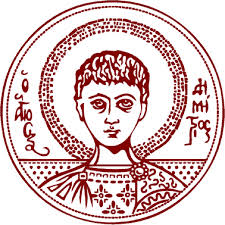
\includegraphics[width=0.2\textwidth]{figures/ap8.jpeg}~\\[1cm]

\textsc{\LARGE Αριστοτέλειο Πανεπιστήμιο Θεσσαλονίκης}\\[1cm]
\textsc{ Πολυτεχνική Σχολή}\\
\textsc{ Τμήμα Ηλεκτρολόγων Μηχανικών και Μηχανικών Υπολογιστών}\\
\textsc{Τομέας Ηλεκτρονικής και Υπολογιστών}\\[1.5cm]

% Title
\HRule \\[0.4cm]
{ \huge \bfseries Υψηλού επιπέδου επίλυση των εξισώσεων συμπιεστής ροής του Euler με την γλώσσα προγραμματισμού Julia\\[0.4cm] }
\HRule \\[2.5cm]

\begin{minipage}[t]{0.48\textwidth}
\textsc{Εκπόνηση Εργασίας:}\\[0.3cm]
\textsc{\Large Ιάσων Μπαρμπαρέσος}
\end{minipage}
\hfill
\begin{minipage}[t]{0.48\textwidth}
\begin{flushright}
\textsc{Επιβλέπων Καθηγητής:}\\[0.3cm]
\textsc{\Large Νικόλαος Πιτσιάνης}
\end{flushright}
\end{minipage}


\vfill

{\Large \textit{Θεσσαλονίκη, 17 Οκτωβρίου 2021}}

\end{center}
\clearpage
 

\end{titlepage}

% \cleardoublepage

%----------------------------------------------------------------------------------------
%	QUOTATION PAGE
%----------------------------------------------------------------------------------------

%----------------------------------------------------------------------------------------
%	ABSTRACT PAGE
%----------------------------------------------------------------------------------------
\vspace*{\fill}  
Ευχαριστίες
\begin{flushright}
Ιάσων Μπαρμπαρέσος
\end{flushright}
\vspace*{\fill}

\newpage


%----------------------------------------------------------------------------------------
%	ACKNOWLEDGEMENTS
%----------------------------------------------------------------------------------------

%----------------------------------------------------------------------------------------
%	LIST OF CONTENTS/FIGURES/TABLES PAGES
%----------------------------------------------------------------------------------------

\listoftodos

\tableofcontents % Prints the main table of contents

\listoffigures % Prints the list of figures

\listoftables % Prints the list of tables

\newpage
\thispagestyle{plain}
\begin{center}
    \textbf{Περίληψη}
\end{center}

\todo[inline]{Write an abstract}



%----------------------------------------------------------------------------------------
%	ABBREVIATIONS
%----------------------------------------------------------------------------------------


%----------------------------------------------------------------------------------------
%	PHYSICAL CONSTANTS/OTHER DEFINITIONS
%----------------------------------------------------------------------------------------


%----------------------------------------------------------------------------------------
%	SYMBOLS
%----------------------------------------------------------------------------------------


%----------------------------------------------------------------------------------------
%	DEDICATION
%----------------------------------------------------------------------------------------


%----------------------------------------------------------------------------------------
%	THESIS CONTENT - CHAPTERS
%----------------------------------------------------------------------------------------

\mainmatter % Begin numeric (1,2,3...) page numbering



\chapter{Εισαγωγή} 

\label{chapter:intro}

\section{Υπολογιστική ρευστομηχανική}

Σε πολλούς τομείς της μηχανικής και της επιστήμης είναι απαραίτητη η πρόβλεψη της συμπεριφοράς ενός ρευστού υπό δεδομένες συνθήκες.
Παρόλο που η συμπεριφορά των ρευστών για τις περισσότερες εφαρμογές περιγράφεται με αρκετά καλή προσέγγιση από της εξισώσεις που προκύπτουν από την μηχανική συνεχούς μέσου, η αναλυτική επίλυση αυτών των εξισώσεων είναι εφικτή μόνο σε ιδιαίτερα απλές γεωμετρίες ή/και μετά από μία σειρά παραδοχών που τις απλοποιούν.

Για την γενική περίπτωση των προβλημάτων που δεν επιδέχονται απλοποιήσεις τέτοιου είδους, παραμένουν δύο επιλογές για την εύρεση του ζητούμενου αποτελέσματος. Η πρώτη είναι η εκτέλεση κάποιου πειράματος, π.χ. σε μία αεροσείραγγα. Αυτή η προσέγγιση, αν και μας επιτρέπει να πάρουμε αρκετά ακριβείς απαντήσεις καθώς δεν χρειάζεται να κάνουμε παραδοχές όσον αφορά την μοντελοποίηση του ρευστού, συνήθως είναι συγκριτικά ακριβότερη οπότε είναι εφικτή μόνο για έναν περιορισμένο αριθμό δοκιμών. Παράλληλα, οι περιορισμοί των συσκευών μέτρησης περιορίζουν τα δεδομένα που μπορούμε να λάβουμε.

Η δεύτερη επιλογή είναι η εκτέλεση μίας υπολογιστικής μελέτης σχετικά με το πρόβλημα. Με την άφιξη οικονομικών και ισχυρών ηλεκτρονικών υπολογιστών διαθέσιμων σε μεμονομένους χρήστες και μικρούς οργανισμούς, αυτή η επιλογή καθίσταται ολοένα και ελκυστικότερη, δεδομένων των περιορισμών κόστους που συνήθως συνοδεύουν μελέτες ανάπτυξης προϊώντων και επιστημονικές μελέτες. Οι υπολογιστικές μελέτες μπορούν να γίνουν με διάφορες τεχνικες, που παρέχουν διαφορετικούς συμβιβασμούς ανάμεσα στο υπολογιστικό κόστος και την ακρίβεια των αποτελεσμάτων.

\section{Παραλληλοποίηση υπολογισμών με κάρτες γραφικών}

Τα περισσότερα προβλήματα υπολογιστικής ρευστομηχανικής, όπως και πληθώρα άλλων προβλημάτων επιστημονικών υπολογισμών, απαιτούν την επανάληψη μίας σειράς βασικών υπολογισμών (iteration) έως την επίτευξη κάποιου κριτηρίου σύγκλισης η τερματισμού του υπολογιστικού πειράματος.
Επιπρόσθετα, πολλές από τις αριθμητικές μεθόδους που χρησιμοποιούνται επιδέχονται σημαντική επιτάχυνση με την παραληλλοποίηση των υπολογισμών τους.

Ο κλασικός τρόπος επίτευξης παραλληλισμού τέτοιου είδους είναι ο καταμερισμός του προβλήματος σε ένα σύνολο υπολογιστών (cluster), εκ των οποίων ο καθένας επιλύει ένα κομμάτι του προβλήματος και επικοινωνεί με τους υπόλοιπους μέσω κάπου προτοκόλου, όπως το δημοφιλές Message Passing Interface (MPI). Αυτή η προσέγγιση, εάν και σε συνδιασμό με της παρακάτω τεχνικές επιτρέπει επίτευξη πολύ μεγάλης κλίμακας (scaling), από μόνη της έχει το μειονέκτημα του υψηλού κόστος ανά παράλληλη μονάδα επεξεργασίας, καθώς και την χρονοβόρα μεταφορά δεδομένων από τον έναν υπολογιστή στον άλλον.

Μία πιο αποδοτική προσέγγιση είναι ο συνδιασμός πολλαπλών πυρήνων επεξεργασίας σε ένα ολοκληρωμένο κύκλωμα, η χρήση δηλαδή πολυπήρηνων επεξεργαστών (multi-core processors). Το κόστος ανά υπολογιστικό πυρήνα είναι σημαντικό μικρότερο σε αυτήν την περίπτωση, ενώ ο κάθε πυρήνας έχει πρόσβαση στην κοινή μνήμη, η προσπέλαση της οποίας είναι αρκετές τάξης μεγέθους γρηγορότερη από την λήψη δεδομένων από άλλους υπολογιστικούς κόμβους, ακόμα και με γρήγορες τεχνολογίες δικτύωσης όπως το InfiniBand.

Τα τελευταία χρόνια, ένας εναλλακτικός τρόπος επιτάχυνσης υπολογισμών με παραλληλοποίηση ήρθε από τον κλάδο των γραφικών υπολογιστών.
Πιο συγκεκριμένα, οι κατασκευαστές καρτών γραφικών, στην προσπάθειά τους να επιτύχουν καλύτερη απόδοση στον σχεδιασμό γραφικών (rendering), κατασκέυασαν επεξεργαστές που μπορούν να επεξεργαστούν έναν μεγάλο αριθμό δεδομένων την ίδια χρονική στιγμή.
Αυτό το μοντέλο υπολογισμών είναι αρκετά χρήσιμο στην γραφική υπολογιστών καθώς σε κάθε καρέ (frame), χρειάζεται να υπολογιστεί το χρώμα για κάθε εικονοστοιχείο (pixel), το οποίο συνήθως προκύπτει ως αποτέλεσμα αλγορίθμων που είναι παρόμοιοι για έναν μεγάλο αριθμό εικονοστοιχείων.
Πέρα από την γραφική όμως, τέτοιου είδους παραλληλισμός (τύπου SIMD όπως θα δούμε σε επόμενο κεφάλαιο), έχει πολλές εφαρμογές σε διάφορους τομείς, με δύο βασικούς να είναι οι επιστημονικοί υπολογισμοί και η εκαίδευση και χρήση νευρωνικών δικτύων σε συστήματα μηχανικής μάθησης (machine learning).

\section{Γλώσσα προγραμματισμού Julia}

Η Julia είναι μία γλώσσα προγραμματισμού της οποίας ο κύριος στόχος είναι η επίλυση του λεγόμενου "προβλήματος των 2 γλωσσών" \cite[p.~67]{Bezanson2017}, το πρόβλημα δηλαδή της αναγκαστικής επιλογής ανάμεσα σε μία γρήγορη γλώσσα χαμηλού επιπέδου (π.χ. C++, Fortran) και μία αργή γλώσσα υψηλού επιπέδου (π.χ. Python).
Η επίλυση αυτού του προβλήματος επιτρέπει σε ερευνητές και μηχανικούς να γράψουν το πρόγραμμά τους μονάχα μία φορά, σε μία γλώσσα η οποία παρέχει εκφραστικότητα υψηλού επιπέδου και την οποία μπορούν να γράψουν και άτομα χωρίς εκτεταμένες γνώσεις προγραμματισμού, ακολουθώντας μερικούς απλούς κανόνες μπορεί να παρέχει απόδοση συγκρίσιμη με γλώσσες χαμηλού επιπέδου.

Η τακτική που ακολουθεί η Julia για τον συνδιασμό αυτών των δύο φαινομενικά ασύμβατων απαιτήσεων, είναι η μεταγλώττιση του κώδικα αμέσως πριν την εκτέλεσή του (JIT compilation), καθώς και η δυνατότητα συγγραφής προγραμμάτων με όσον τον δυνατό γίνεται πιο γενικό τρόπο, γεγονός που επιτρέπει τον εύκολο συνδιασμό τους.

Όπως θα δούμε και στην συνέχεια, το στυλ προγραμματισμού της Julia ταιριάζει αρκετά στις ανάγκες του προγραμματισμού καρτών γραφικών \cite{Besard2019b}.
Η υποστήριξη προγραμματισμού καρτών γραφικών παρέχεται από τα πακέτα της ομάδας JuliaGPU: για τις κάρτες γραφικών της NVIDIA το CUDA.jl (πρώην CUDAdrv.jl, CUDAnative.jl, και CuArrays.jl) \cite{Besard2019a}, για αυτές της AMD το AMDGPU.jl, και για τους επιταχυντές της Intel το oneAPI.jl.

\section{Στόχοι της διπλωματικής εργασίας}

Παρόλο που οι δυνατότητες προγραμματισμού καρτών γραφικών για επιστημονικούς υπολογισμούς είναι διαθέσιμοι εδώ και αρκετά χρόνια, τα πιο γνωστά εμπορικά πακέτα υπολογιστικής ρευστομηχανικής είτε αξιοποιούν επιτάχυνση με κάρτες γραφικών μόνο για τους επιλυτές γραμμικών συστημάτων τους (ANSYS Fluent, OpenFOAM), είτε δεν παρέχουν κάποια δυνατότητα επιτάχυνσης καθόλου (SU2 \cite{Palacios2013}).

\todo{Citation needed}

Ο κύριος στόχος της παρούσας διπλωματικής εργασίας είναι να ερευνήσει κατά πόσο το νέο στυλ προγραμματισμού που παρέχεται από την Julia, σε συνδιασμό με τις δυνατότητες μοντέρνων καρτών γραφικών μπορεί να παρέχει μία πλατφόρμα για την επίλυση προβλημάτων υπολογιστικής ρευστομηχανικής, η οποία είναι εύκολη στην χρήση και την τροποποίηση, αλλά παράλληλα εκμεταλλεύεται πλήρως τις δυνατότητες του διαθέσιμου υλικού και πετυχαίνει απόδοση συγκρίσιμη με αυτή των πλέον γνωστών πακέτων υπολογιστικής ρευστομηχανικής.

Αν και προσπάθειες σχεδίασης μίας γλώσσας προγραμματισμού συγκεκριμένα για παράλληλους υπολογισμούς έχουν γίνει στο παρελθόν (Futhark \cite{Henriksen2017}), καθώς και γλωσσών συγκεκριμένα για υπολογισμούς σε γεωμετρικά πλέγματα (meshes) για επίλυση μερικών διαφορικών εξισώσεων (PDEs) (Liszt), θεωρούμε ότι οι δυνατότητες σύνθεσης προγραμμάτων της Julia επιτρέπουν την επίτευξη ενός υψηλού επιπέδου εκφραστηκότητας χωρίς να απαιτούν την χρήση μίας γλώσσας DSL.

Υπάρχουν ήδη διάφορες προσπάθειες για την ανάπτυξη πακέτων επίλυσης PDE με Julia αλλά μέχρι στιγμής κανένα δεν υποστηρίζει μη δομημένα πλέγματα (unstructured meshes) τα οποία κατά βάσει χρησιμοποιούνται σε εφαρμογές μηχανολογίας, ενώ τα περισσότερα εστιάζουν σε γενικά μαθηματικά προβλήματα και δεν παρέχουν συναρτήσεις για την γρήγορα επίλυση προβλημάτων ρευστομηχανικής.

\todo{Cite Liszt and perhaps refine the limitation of other Julia packages}

\section{Οργάνωση κειμένου}

\todo[inline]{Briefly describe the scope of each chapter. Perhaps this should be done after most chapters have some content.}


\chapter{Θεωρητικό υπόβαθρο}
\label{chapter:theory}

\section{Υπολογιστική ρευστομηχανική}

Όπως αναφέρθηκε και στην εισαγωγή, η υπολογιστική ρευστομηχανική αναφέρεται στην επίλυση προβλημάτων ρευστομηχανικής με αριθμητικές μεθόδους.
Σε αυτήν την ενότητα θα ασχοληθούμε με την φυσική μοντελοποίηση των προβλημάτων που θέλουμε να λύσουμε, βήμα απαραίτητο πριν προχωρήσουμε στην αριθμητική μέθοδο.

Αρχικά, αξίζει να αναφέρουμε ότι στην παρούσα εργασία ασχολούμαστε με την περιγραφή των ρευστών σε μακροσκοπική κλίμακα.
Αυτό σημαίνει ότι θεωρούμε ότι μπορούμε να περιγράψουμε το ρευστό ως ένα \emph{συνεχές μέσο} (continuum) με σημειακές ιδιότητες (πυκνότητα, ταχύτητα, πίεση κλπ), χωρίς να ασχολούμαστε με την μοριακή φύση του ρευστού.

Απαραίτητη προϋπόθεση για αυτήν την παραδοχή είναι η κλίμακα του προβλήματος να είναι σημαντικά μεγαλύτερη από την μέση ελεύθερη διαδρομή (mean free path).
Μία αποδεκτή ποσοτικοποίηση αυτής της συνθήκης είναι να ισχύει $\mathrm{Kn} < 0.01$, όπου $\mathrm{Kn}$ ο αριθμός \emph{Knudsen} που ορίζεται ως:

\begin{equation*}
    \mathrm{Kn} = \frac{\lambda}{L}
\end{equation*}

όπου $\lambda$ η μέση ελεύθερη διαδρομή (mean free path) και L ένα χαρακτηριστικό μήκος του προβλήματος υπό μελέτη.

Με την παραδοχή αυτή του συνεχούς μέσου, η μοντελοποίηση της κίνησης των ρευστών κατά βάσει γίνεται με την εξίσωση ορμής Navier-Stokes, οι οποία σε σημειακή μορφή (point form) έχει την εξής μορφή:

\todo{Citation for NS}

\begin{equation}
    \rho \frac{\mathrm{D} \mathbf{u}}{\mathrm{D}t} = \nabla \cdot \mathbf{\sigma} + \mathbf{f}
    \label{eq:cauchy}
\end{equation}

όπου:

\begin{itemize}
    \item $\rho$ είναι η πυκνότητα,
    \item $\mathbf{u}$ είναι το διάνυσμα της ταχύτητας,
    \item $\frac{\mathrm{D}}{\mathrm{D}t} = (\mathbf{u} \cdot \nabla )$ είναι η υλική παράγωγος (material derivative),
    \item $\mathbf{\sigma}$ είναι ο τανυστής της τάσης (stress tensor), και
    \item $\mathbf{f}$ είναι η τοπική δύναμη που τυχόν ασκείται σε κάθε σημείο του ρευστού, π.χ. για ένα ρευστό σε σταθερό, ομοιόμορφο βαρυτικό πεδίο $\mathbf{f} = \rho \mathbf{g}$ όπου $\mathbf{g}$ το διάνυσμα της βαρυτικής επιτάχυνσης.
\end{itemize}

Αυτή η εξίσωση περιγράφει την διατήρηση/μεταβολή της ορμής του ρευστού.
Για τον πλήρη ορισμό του προβλήματος και την επίλυσή του, χρειάζεται επίσης να ορίσουμε δύο ακόμη εξισώσεις.
Αυτές κατά κανόνα είναι:

\begin{itemize}
    \item Μία εξίσωση που προκύπτει από την αρχή διατήρησης της μάζας, εφόσον μπορούμε να κάνουμε μία τέτοια υπόθεση:
        \begin{equation*}
            \frac{\partial \rho}{\partial t} + \nabla \cdot \left( \rho \mathbf{u} \right) = 0
        \end{equation*}
    \item Μία εξίσωση που προκύπτει από την διατήρηση της ενέργειας.
\end{itemize}

Αυτές οι τρεις εξισώσεις μαζί συνήθως αναφέρονται ως οι \emph{εξισώσεις Navier-Stokes}.

Αν και οι εξισώσεις Navier-Stokes περιγράφουν την συμπεριφορά των ρευστών σε ένα πολύ μεγάλο εύρος προβλημάτων, είναι συνηθισμένο να χωρίζουμε τα προβλήματα σε υποκατηγορίες προκειμένου να επιλέξουμε έναν κατάλληλο αλγόριθμο επίλυσης.
Ένα κριτήριο διαχωρισμού είναι η τάξη μεγέθους του αριθμού Reynolds της ροής, που ορίζεται ως:

\begin{equation*}
    \mathrm{Re} = \frac{\rho U_{\infty} L}{\mu} = \frac{U_\infty L}{\nu}
\end{equation*}

όπου:

\begin{itemize}
    \item $\rho$ είναι η πυκνότητα του ρευστού,
    \item $U_{\infty}$ είναι η ταχύτητα ελεύθερης ροής,
    \item $L$ είναι το χαρακτηριστικό μήκος του προβλήματος,
    \item $\mu$ είναι το ιξώδες, και
    \item $\nu$ είναι το κινηματικό ιξώδες (kinematic viscosity) $\nu = \mu / \rho$.
\end{itemize}

Στην παρούσα εργασία θα ασχοληθούμε με μία υποκατηγορία προβλημάτων για την οποία $\mathrm{Re} \to \infty$.
Πρακτικά αυτό σημαίνει ότι η αδράνεια του ρευστού έχει πολύ μεγαλύτερη επιρροή στην συμπεριφορά του από ότι το ιξώδες, και συνεπώς μπορούμε να αγνοήσουμε την επιρροή του δεύτερου στο μοντέλο μας.
Αν και αυτή η παραδοχή μπορεί να φαίνονται αυθαίρετη, είναι μία καλή προσέγγιση στην περίπτωση διηχητικών και υπερηχητικών αεροδυναμικών ροών.
Η προσέγγιση παύει να είναι ικανοποιητική καθώς η ροή γίνεται υπερυπερηχητική (hypersonic), δηλαδή για αριθμό Mach μεγαλύτερο από 5, όπου φαινόμενα όπως ο ιονισμός του αερίου αρχίζουν να γίνονται σημαντικά.

Μία άλλη κατηγοριοποίηση που μπορούμε να κάνουμε, είναι αυτή της \emph{συμπιεστότητας} (compressibility) του ρευστού.
Για την περίπτωση των υγρών αλλά και ροών αερίων με αριθμό Mach μικρότερο από 0.3, μπορούμε πολλές φορές να θεωρήσουμε ότι η πυκνότητα είναι σταθερή.
Με αυτήν την παραδοχή, η εξίσωση διατήρησης της μάζας γίνεται

\begin{equation*}
    \nabla \cdot \mathbf{u} = 0
\end{equation*}

δηλαδή το πεδίο της ταχύτητας είναι ασυμπίεστο.
Σε αυτήν την περίπτωση οι μέθοδοι επίλυσης είναι διαφορετικοί, καθώς χρειάζεται να βρεθεί ένας τρόπος να υπολογιστεί η αλλαγή του πεδίου πίεσης, η οποία διαφορετικά προκύπτει από την εξίσωση κατάστασης του αερίου.
Μία γνωστή μέθοδος είναι η μέθοδος SIMPLE.

Όπως αναφέραμε προηγουμένως όμως, στην παρούσα θα ασχοληθούμε με την επίλυση προβλημάτων ροής για τα οποία ο αριθμός Mach είναι μεγαλύτερος από 0.3, καθώς μιλάμε για διηχητικές και υπερηχητικές ροές, και συνεπώς θα θεωρήσουμε ότι το αέριο είναι συμπιεστό.

\section{Συμπιεστή ροή χωρίς ιξώδες}

Πριν προχωρήσουμε στην μαθηματική περιγραφή των συμπιεστών ροών χωρίς ιξώδες, αξίζει να αναφέρουμε ένα φυσικό χαρακτηριστικό των συμπιεστών ροών με αριθμό Mach κοντά ή πάνω από 1, το οποίο θα πρέπει να λάβουμε υπόψιν μας στην σχεδίαση του αλγόριθμου επίλυσης.

Το φαινόμενο αυτό είναι το λεγόμενο \emph{κρουστικό κύμα} (shockwave), το οποίο αναφέρεται σε μία απότομη αλλαγή στις τιμές των ροϊκών πεδίων που σχηματίζεται όταν μία διαταραχή μεταδίδεται γρηγορότερα από την τοπική ταχύτητα του ήχου.
Ένα τυπικό παράδειγμα είναι τα κρουστικά κύματα που σχηματίζονται πάνω στις ακμές προσβολής (leading edge) των πτερυγίων υπερηχητικών αεροσκαφών, η τα σφαιρικά κύματα που σχηματίζονται με την ανατίναξη (detonation) μίας ποσότητας εκρηκτικών υλών.
Τα κρουστικά κύματα έχουν πολύ μικρό πάχος (συγκρίσιμο με την μέση ελεύθερη διαδρομή), και συνεπώς κατά την μαθηματική περιγραφή της λύσης μας χρειάζεται να τα αντιμετωπίσουμε ως ασυνέχειες.

Η μαθηματική περιγραφή συμπιεστών ροών χωρίς ιξώδες προκύπτει από τις εξισώσεις Navier-Stokes εάν αγνοήσουμε τους όρους του ιξώδους.
Με άλλα λόγια, θεωρούμε ότι η μοναδική δύναμη που ασκείται στο ρευστό είναι αυτή της πίεσης, δηλαδή ο τανυστής τάσης $\sigma$ γίνεται:

\begin{equation*}
    \mathbf{\sigma} = -p\mathbf{I} \Rightarrow \nabla \cdot \mathbf{\sigma} = -\nabla p
\end{equation*}

Θα θεωρήσουμε επίσης ότι η ροή είναι αδιαβατική, η επίδραση της βαρύτητας είναι αμελητέα και ότι δεν υπάρχει κάποιο άλλο πεδίο δύναμης που να ασκεί δύναμη στο ρευστό, δηλαδή $\mathbf{f} = 0$.
Συνδιάζοντας έτσι την \eqref{eq:cauchy} με την εξίσωση διατήρησης της μάζας και μία εξίσωση διατήρησης ενέργειας που προκύπτει από τον πρώτο νόμο της θερμοδυναμικής, προκύπτουν οι \emph{εξισώσεις του Euler}, σε σημειακή μορφή:

\begin{align}\label{eq:euler}
    \frac{\mathrm{D}\rho}{\mathrm{D}t} &= -\rho \nabla \cdot \mathbf{u} \\
    \frac{\mathrm{D} \mathbf{u}}{\mathrm{D}t} &= -\frac{\nabla p}{\rho} \\
    \frac{\mathrm{D} e_i}{\mathrm{D}t} &= -\frac{p}{\rho} \nabla \cdot \mathbf{u}
\end{align}

όπου $e_i$ η εσωτερική ενέργεια του αερίου ανα μονάδα μάζας, $e_i = c_v T$ όπου $T$ η απόλυτη θερμοκρασία.

Χρειαζόμαστε όμως μία ακόμη εξίσωση για τον υπολογισμό της πίεσης.
Ορίζοντας την συνολική ενέργεια ανα μονάδα μάζας $e = e_i + \frac{1}{2} |\mathbf{u}|^2$, για ιδανικά αέρια έχουμε

\begin{align*}
    p &= \rho R T \\
      &= \rho R \frac{e - \frac{1}{2} \mathbf{u}|^2}{c_v} \\
      &= \rho R \frac{\gamma - 1}{R} \left( e - \frac{1}{2} |\mathbf{u}|^2 \right) \\
      &= \rho \left(\gamma - 1\right) \left( e - \frac{1}{2} |\mathbf{u}|^2 \right) \\
\end{align*}

όπου $R$ η \emph{ειδική θερμοδυναμική σταθερά} (specific gas constant) και $\gamma = c_p / c_v$ ο λόγος των ειδικών θερμοτήτων (specific heat ratio).

Μπορούμε επίσης να εκφράσουμε τις εξισώσεις ως ένα πρόβλημα διάχυσης, όπου μία ποσότητα $\mathbf{U}$ διαχέεται με το διάνυσμα ροής (flux) $\mathbf{F}$, δηλαδή

\begin{equation*}
    \frac{\partial \mathbf{U}}{\partial t} + \nabla \cdot \mathbf{F} = 0
\end{equation*}

όπου

\begin{equation*}
    \mathbf{U} = 
        \begin{bmatrix}
            \rho \\
            \rho \mathbf{u} \\
            \rho e
        \end{bmatrix}
    , \ 
    \mathbf{F} =
        \begin{bmatrix}
            \rho \mathbf{u} \\
            \mathbf{u} \otimes \left( \rho \mathbf{u} \right) + p \mathbf{I} \\
            (e + p) \mathbf{u}
        \end{bmatrix}
\end{equation*}

ή, για την περίπτωση των δύο διαστάσεων που θα μας απασχολήσει και στην συνέχεια

\begin{equation*}
    \frac{\partial \mathbf{U}}{\partial t} + \frac{\partial \mathbf{F}}{\partial x} + \frac{\partial \mathbf{G}}{\partial y} = 0
\end{equation*}

όπου

\begin{equation*}
    \mathbf{U} = 
        \begin{bmatrix}
            \rho \\
            \rho u \\
            \rho v \\
            \rho e
        \end{bmatrix}
    , \ 
    \mathbf{F} =
        \begin{bmatrix}
            \rho u \\
            \rho u^2 + p \\
            \rho u v \\
            (e + p) u
        \end{bmatrix}
    , \ 
    \mathbf{G} =
        \begin{bmatrix}
            \rho v \\
            \rho u v \\
            \rho v^2 + p \\
            (e + p) v 
        \end{bmatrix}
\end{equation*}
.

\section{Η μέθοδος πεπερασμένων όγκων 1ης τάξης}

Οι παραπάνω εξισώσεις περιγράφουν την συμπεριφορά ενός ρευστού σε κάθε σημείο.
Για να είναι το πρόβλημα καλά ορισμένο (well-posed) χρειάζεται επίσης να ορίσουμε τις οριακές συνθήκες που πρέπει να ικανοποιεί η λύση, και κατά συνέπεια να ορίσουμε πλήρως τον χώρο (domain) στον οποίο η λύση ορίζεται.

Έστω λοιπόν ότι η λύση ενός τέτοιο προβλήματος είναι η συνάρτηση $U$ η οποία ορίζεται σε κάθε σημείο ενός πεπερασμένου χώρου $\Omega \in \mathbb{R}^2$.
Με άλλα λόγια $U : \Omega \rightarrow \mathbb{R}^n$ όπου $n$ ο αριθμός των βαθμωτών πεδίων που ορίζουν την λύση.
Για τις εξισώσεις Euler σε δύο διαστάσεις όπως ορίζονται στην προηγούμενη ενότητα $n = 4$.

Για την αριθμητική προσέγγιση της λύσης $U$, το πρώτο βήμα είναι να βρούμε έναν τρόπο αναπαράστασης της λύσης με έναν πεπερασμένο αριθμό (έστω $N$) συντελεστών, έτσι ώστε αυτή να μπορεί να αποθηκευθεί και να επεξεργαστεί από έναν ηλεκτρονικό υπολογιστή.
Έστω $U_i \in \mathbb{R}^n$ ο συντελεστής $i$.
Μπορούμε να ορίσουμε την αριθμητική προσέγγιση της λύσης $\hat{U}$ ως τον γραμμικό συνδιασμό $N$ συναρτήσεων βάσης $\phi_i : \Omega \rightarrow \mathbb{R}$:

\begin{equation}
    \hat{U} = \sum_{i = 0}^{N} U_i \phi_i
\end{equation}

Εάν $V$ ο διανυσματικός χώρος (vector space) όλων των συναρτήσεων από το $\Omega$ στο $\mathbb{R}^n$, τότε, για πεπερασμένο $N$, οι συναρτήσεις βάσης ορίζουν έναν υποχώρο του $V$, και άρα η αριθμητική προσέγγιση $\hat{U}$ δεν μπορεί να αναπαραστήσει πλήρως την πραγματική λύση $U$ εκτός και αν αυτή βρίσκεται στον υποχώρο που ορίζουν οι συναρτήσεις βάσης.

Για να ορίσουμε της συναρτήσεις βάσης που θα χρησιμοποιήσουμε στην μέθοδο πεπερασμένων όγκων, ξεκινάμε χωρίζοντας τον χώρο $\Omega$ σε $N$ υποχώρους $S_i$ έτσι ώστε:

\begin{equation}
    \Omega = \bigcup_{i = 0}^{N} S_i
\end{equation}

Τους υποχώρους αυτούς θα τους αποκαλούμε \emph{πεπερασμένους όγκους} (finite volumes) ή \emph{κελιά} (cells).

Μπορούμε να ορίσουμε τώρα τις συναρτήσεις βάσης της μεθόδου πεπερασμένων όγκων πρώτης τάξης ως:

\begin{equation}
    \phi_i(\mathbf{x}) =
        \begin{cases}
            1 & \mathbf{x} \in S_i \\
            0 & \mathbf{x} \notin S_i
        \end{cases}
\end{equation}

Πρακτικά αυτό σημαίνει ότι υποθέτουμε ότι η λύση είναι σταθερή στο εσωτερικό κάθε πεπερασμένου όγκου, αλλά ασυνεχής ανάμεσά τους.
Καθώς η προσέγγιση $\hat{U}$ είναι γραμμικός συνδιασμός αυτών των μη συνεχών συναρτήσεων βάσης, η προσέγγιση θα είναι και αυτή ασυνεχής.

\begin{figure}
    \centering
    \tdplotsetmaincoords{70}{80}
    \begin{tikzpicture}[scale=2, tdplot_main_coords]
        \coordinate (A) at (-2, -1.3, 0);
        \coordinate (B) at (1, -1, 0);
        \coordinate (C) at (-1, 1, 0);
        \coordinate (D) at (1.5, 1.5, 0);
        \coordinate (Ah) at (-2, -1.3, 2.0);
        \coordinate (Bh) at (1, -1, 2.0);
        \coordinate (Ch) at (-1, 1, 2.0);
        \coordinate (Bl) at (1, -1, 1.2);
        \coordinate (Cl) at (-1, 1, 1.2);
        \coordinate (Dl) at (1.5, 1.5, 1.2);

        \coordinate (S1) at (-0.67, -0.43, 0);
        \coordinate (S1h) at (-0.67, -0.43, 2.0);

        \coordinate (S2) at (0.5, 0.5, 0);
        \coordinate (S2h) at (0.5, 0.5, 1.2);


        \draw[dashed] (A) -- (B) -- (C) -- cycle;
        \draw[dashed] (C) -- (D) -- (B);

        \draw (Ah) -- (Bh) -- (Ch) -- cycle;
        \draw (Bl) -- (Cl) -- (Dl) -- cycle;

        \draw[dotted] (Ah) -- (A) (Bl) -- (B) (Cl) -- (C) (Dl) -- (D);
        \draw (Bh) -- (Bl) (Ch) -- (Cl);

        \draw (S1) node{$S_1$} (S2) node{$S_2$};
        \draw (S1h) node{$U_1 \phi_1$} (S2h) node{$U_2 \phi_2$};

        \draw (Ch) +(0, 0, -0.4) node[right]{$\hat{U} = \sum_i^N U_i \phi_i$};
    \end{tikzpicture}
    \caption{Στην μέθοδο πεπερασμένων όγκων πρώτης τάξης υποθέτουμε ότι η λύση είναι σταθερή σε κάθε πεπερασμένο όγκο. Αυτό οδηγεί στον σχηματισμό ασυνεχειών στην επιφάνεια της λύσης $\hat{U}$ στα όρια ανάμεσα στους πεπερασμένους όγκους, αλλά επιτρέπει επίσης την καλή αναπαράσταση ασυνεχειών στην λύση όπως είναι π.χ. τα κρουστικά κύματα.}
    \label{fig:fvm-basis}
\end{figure}

Παραμένει όμως το πρόβλημα υπολογισμού των συντελεστών $U_i$.
Οι συντελεστές αυτοί είναι συναρτήσεις του χρόνου, καθώς μέχρι στιγμής έχουμε διακριτοποιήσει το πρόβλημα μόνο στον χώρο.
Η μέθοδος πεπερασμένων όγκων θα μας επιτρέψει να κατασκευάσουμε ένα σύστημα διαφορικών εξισώσεων που περιγράφει την χρονική εξέλιξη αυτών των συντελεστών, και μας δίνει σε κάθε χρονική στιγμή έναν τρόπο υπολογισμού των χρονικών παραγώγων $\frac{\mathrm{d}U_i}{\mathrm{d}t}$.
Με τις χρονικές παραγώγους διαθέσιμες, μπορούμε να λύσουμε το σύστημα διαφορικών εξισώσεων που προκύπτει με έναν από τους πολλούς αλγόριθμους χρονικής ολοκλήρωσης που υπάρχουν, επιλύοντας είτε μέχρι μία χρονική στιγμή $t_1$, για την περίπτωση ενός μεταβατικού προβλήματος (transient problem), είτε μέχρι οι χρονικές παράγωγοι να πλησιάσουν ικανοποιητικά κοντά στο μηδέν για ένα πρόβλημα μόνιμης κατάστασης (steady state problem).
Υπάρχουν πολλοί τέτοιοι αλγόριθμοι, με τον πιό απλό να είναι ο αλγόριθμος χρονικής ολοκλήρωσης του Euler όπου $u^{t + 1} = u^{t} + \frac{\mathrm{d} u}{\mathrm{d}t} \mathrm{d} t$.
Καθώς η επιλογή αυτή δεν αλλάζει την μέθοδο υπολογισμού των παραγώγων που θα περιγράψουμε παρακάτω, στο σημείο αυτό δεν θα επεκταθούμε περαιτέρω στο θέμα της χρονικής ολοκλήρωσης.

Η μέθοδος πεπερασμένων όγκων μας επιτρέπει να επιλύσουμε προβλήματα της μορφής

\begin{equation}
    \label{eq:advection-point-form}
    \frac{\partial \mathbf{U}}{\partial t} + \nabla \cdot \mathbf{F} = 0
\end{equation}

Η εξίσωση αυτή θα πρέπει να ισχύει σε κάθε σημείο του χώρου $\Omega$ και, κατά συνέπεια, σε κάθε σημείο ενός πεπερασμένου όγκου $S_i$ για κάθε $i$.
Ολοκληρώνοντας την εξίσωση \eqref{eq:advection-point-form} στο εσωτερικό ενός πεπερασμένου όγκου $S_i$ έχουμε:

\begin{equation*}
    \label{eq:fvm-int}
    \int_{S_i} \left( \frac{\partial U}{\partial t} + \nabla \cdot \mathbf{F} \right) \mathrm{d} S = 
    \int_{S_i} \frac{\partial U}{\partial t} \mathrm{d} S
    + \int_{S_i} \left( \nabla \cdot \mathbf{F} \right) \mathrm{d} S = 0
\end{equation*}

Ξεκινώντας με τον πρώτο όρο της εξίσωσης \eqref{eq:fvm-int}, και θυμίζοντας ότι $U = \sum_{i = 0}^N U_i \phi_i$, έχουμε:

\begin{align}
    &\int_{S_i} \frac{\partial U}{\partial t} \mathrm{d} S \notag \\
    = &\int_{S_i} \frac{\partial}{\partial t}\left( \sum_{j = 0}^{N} U_j \phi_j \right) \mathrm{d} S \notag \\
    = &\int_{S_i} \frac{\partial}{\partial t}\left( U_i \phi_i \right) \mathrm{d} S \quad \text{καθώς $\phi_j = 0$ αν $i \neq j$} \notag \\
    = &A \frac{\mathrm{d}U_i}{\mathrm{d}t} \quad \text{καθώς $\phi_i = 1$ στο εσωτερικό του $S_i$} \label{eq:fvm-lhs}
\end{align}

όπου $A = \int_{S_i} \mathrm{d} S$ η επιφάνεια (ή όγκος στις τρεις διαστάσεις) του πεπερασμένου όγκου $S_i$.

Συνεχίζοντας με τον δεύτερο όρο της εξίσωσης \eqref{eq:fvm-int}, χρησιμοποιώντας το θεώρημα της απόκλισης (divergence theorem) έχουμε:

\begin{equation}
    \label{eq:fvm-rhs}
    \int_{S_i} \left( \nabla \cdot \mathbf{F} \right) \mathrm{d} S 
    = \oint_{\partial S_i} \left( \mathbf{F} \cdot \mathbf{n} \right) \mathrm{d} l
\end{equation}

όπου $\mathbf{n}$ είναι ένα διάνυσμα κάθετο στο όριο $\partial S_i$ με μήκος 1, και $l$ το διαφορικό μήκους (ή επιφανείας στις τρεις διαστάσεις).

Συνδιάζοντας τις εξισώσεις \eqref{eq:fvm-lhs} και \eqref{eq:fvm-rhs} έχουμε την εξής σχέση για τον υπολογισμό της χρονικής παραγώγου του συντελεστή $U_i$:

\begin{equation}
    \label{eq:fvm-update-cont}
    \frac{\mathrm{d} U_i}{\mathrm{d} t} = -\frac{1}{A} \oint_{\partial S_i} \left( \mathbf{F} \cdot \mathbf{n} \right) \mathrm{d} l
\end{equation}

Εδώ όμως έχουμε ένα ακόμη πρόβλημα: Η συνάρτηση της ροής $\mathbf{F}$ είναι συνήθως συνάρτηση της λύσης $U$, αλλά η προσέγγιση της λύσης είναι ασυνεχής πάνω στο όριο ανάμεσα σε δύο πεπερασμένους όγκους.
Χρειάζεται να βρούμε έναν τρόπο λοιπόν, να αντικαταστήσουμε την συνάρτηση $\mathbf{F}(U)$ με μία άλλη $\mathbf{F}\left(U_1, U_2\right)$ που υπολογίζει την ροή λαμβάνοντας υπόψιν τις τιμές της λύσης στις 2 πλευρές του ορίου πάνω στο οποίο ολοκληρώνουμε.

Μία γνωστή μέθοδος, είναι η μέθοδος Godunov \cite[p. ~105]{Knight2006}. Αν εστιάσουμε πάνω σε ένα σημείο του ασυνεχούς ορίου, και αγνοήσουμε προς το παρόν τους υπόλοιπους πεπερασμένους όγκους, μπορούμε να θεωρήσουμε ότι έχουμε ένα μονοδιάστατο πρόβλημα αρχικών τιμών (initial value problem/IVP), του οποίου η λύση είναι η εξέλιξη στον χρόνο μιας τέτοιας ασυνέχειας.
Το πρόβλημα αυτό λέγεται \emph{πρόβλημα Riemann}, και υπάρχουν αρκετοί αλγόριθμοι επίλυσής του, είτε ακριβώς (π.χ. Godunov), είτε προσεγγιστικά (π.χ. μέθοδος Roe με γραμμικοποίηση, HLLC, HLLE, κ.α.).
Οι αλγόριθμοι αυτοί έχουν ως αποτέλεσμα τον υπολογισμό της ροής $\mathbf{F}\left(U_1, U_2\right)$ που ψάχνουμε, με έναν αναπόφευκτο συμβιβασμό ανάμεσα σε ταχύτητα και ακρίβεια.

Μία άλλη μέθοδος είναι αυτή του διαχωρισμού των διανυσμάτων εκροής (Flux Vector Splitting/FVS).
Εδώ χωρίζουμε την ροή $\mathbf{F}$, σε δύο διανύσματα ως εξής:

\begin{equation}
    \mathbf{F} = \mathbf{F}_{+} + \mathbf{F}_{-}
\end{equation}

όπου:
\begin{itemize}
    \item $\mathbf{F}_{+}$ είναι η ροή που προκύπτει από την διάδοση κυμάτων στην θετική κατεύθηνση (έξω από τον όγκο ελέγχου), και
    \item $\mathbf{F}_{-}$ είναι η ροή που προκύπτει από την διάδοση κυμάτων στην αρνητική κατεύθηνση (προς το εσωτερικό του όγκου ελέγχου)
\end{itemize}

Για τον χωρισμό των διανυσμάτων εκροής, χρειάζεται να βρούμε της χαρακτηριστικές (characteristics) της εξίσωσης, οι οποίες μας δίνουν την κατεύθηνση και ταχύτητα διάδοσης των κυμάτων.
Για τις εξισώσεις Euler σε μία διάσταση, προκύπτουν τρεις ταχύτητες διάδοσης $u$, $u + \alpha$, και $u - \alpha$, όπου $u$ η ταχύτητα της ροής στην θετική κατεύθηνση και $\alpha$ η τοπική ταχύτητα του ήχου.
Υπάρχουν πολλοί αλγόριθμοι που βασίζονται στην μέθοδο FVS \cite{Toro2012}.

Για τις υπολογιστικές μελέτες της παρούσας εργασίας θα χρησιμοποιήσουμε την μέθοδο χωρισμού διανυσμάτων εκροής AUFS \cite{Sun2003}, αλλά η υπολογιστική μέθοδος της εργασίας επιτρέπει την χρήση άλλων μεθόδων υπολογισμού του $\mathbf{F}$ χωρίς ιδιαίτερο κόπο.

Βλέπουμε λοιπόν ότι η μέθοδος πεπερασμένων όγκων μας παρέχει τόσο μία επιλογή συναρτήσεων βάσης αλλά και μία μέθοδο υπολογισμού των συντελεστών $U_i$ έτσι ώστε η προσέγγιση $\hat{U}$ να είναι μία καλή προσέγγιση της πραγματικής λύσης $U$.
Η μετατροπή αυτή ενός συστήματος μερικών διαφορικών εξισώσεων (PDE) σε έναν σύστημα απλών διαφορικών εξισώσεων (ODE) και η επίλυση αυτού με συμβατικές μεθόδους είναι επίσης γνωστή ως η \emph{μέθοδος των γραμμών} (method of lines) \cite[p. ~352]{Solomon2015}.

Αν και δεν υπάρχει κάποιος θεωρητικός περιορισμός όσον αφορά το σχήμα των πεπερασμένων όγκων, στην πράξη χρησιμοποιούνται κατά βάση πολύγωνα.
Για προβλήματα δύο διαστάσεων, συνήθης επιλογές είναι τα τρίγωνα (λόγω απλότητας και ύπαρξης μεγάλης πληθώρας αλγορίθμων τριγωνοποίησης, π.χ. Delauney), τα τετράγωνα (κυρίως σε δομημένα πλέγματα (structured grids)), και τα εξάγωνα (λόγω δυνατότητας κάλυψης του χώρου με μικρότερο αριθμό κελιών).

\begin{figure}
    \centering
    \begin{tikzpicture}[scale=1.5]
        \coordinate (A) at (-2, -1.3);
        \coordinate (B) at (1, -1);
        \coordinate (C) at (-1, 1);
        \coordinate (D) at (1.5, 1.5);
        \coordinate (CB) at (0, 0);
        \coordinate (AB) at (-0.5, -1.15);
        \coordinate (AC) at (-1.5, -0.15);

        \draw (A) -- (B) -- (C) -- cycle;
        \draw (C) -- (D) -- (B);

        \draw[dashed] (C) -- +(80:1) (C) -- +(160:1)
            (A) -- +(110:1) (A) -- +(170:1) (A) -- +(230:1) (A) -- +(300:1)
            (B) -- +(240:1) (B) -- +(330:1) (B) -- +(20:1)
            (D) -- +(320:1) (D) -- +(0:1) (D) -- +(60:1) (D) -- +(130:1);

        \fill (CB) circle[radius=0.05] (AB) circle[radius=0.05] (AC) circle[radius=0.05];

        \draw[-{Stealth[scale=2]}] (AB) -- +(0.06, -0.6) node[below]{$\mathbf{\hat{n}}_1$};
        \draw[-{Stealth[scale=2]}] (CB) -- +(0.5, 0.5) node[below right]{$\mathbf{\hat{n}}_2$};
        \draw[-{Stealth[scale=2]}] (AC) -- +(-0.575, 0.25) node[above]{$\mathbf{\hat{n}}_3$};

        \draw (AB) +(-0.25, 0.5) node[above]{$S_i$};

        \draw (CB) +(-0.5, 0.5) node[below left]{$U_i$};
        \draw (CB) +(-0.5, 0.5) node[above right]{$U_{+,2}$};

        \draw (CB) +(0.05, 0) node[right]{$L_2$};
        \draw (AB) node[above]{$L_1$};
        \draw (AC) node[below right]{$L_3$};
        \draw[-{Stealth[scale=2]}] (CB) -- +(0.4, 0.8) node[above right]{$\mathbf{F}$};
    \end{tikzpicture}
    \caption{Σχηματική αναπαράσταση του υπολογισμού της ροής ανάμεσα σε δύο γειτονικά τριγωνικά στοιχεία στον διδιάστατο χώρο.}
    \label{fig:fvm-triangle-flux}
\end{figure}

Η χρήση πολυγώνων κάνει τον υπολογισμό του ολοκληρώματος της εξίσωσης \eqref{eq:fvm-update-cont} ιδιαίτερα εύκολο. Τόσο οι τιμές της λύσης που χρησιμοποιούνται στον υπολογισμό του $\mathbf{F}$, τόσο και το μοναδιαίο διάνυσμα $\mathbf{\hat{n}}$ στο οποίο προβάλλουμε το διάνυσμα ροής $\mathbf{F}$ είναι σταθερά κατά μήκος τις κάθε πλευράς του πολυγώνου. Ο τρόπος υπολογισμού της ροής σε κάθε πλευρά ενός τριγώνου στο διδιάστατο χώρο φαίνεται στο σχήμα \ref{fig:fvm-triangle-flux}. Έτσι το ολοκλήρωμα μετατρέπεται σε απλό άθροισμα, με έναν όρο για κάθε πλευρά του πολυγώνου:

\begin{equation}
    \frac{\mathrm{d} U_i}{\mathrm{d} t} = -\frac{1}{A_i}
    \sum_{j = 0}^{K} \mathbf{F} \left( U_i, U_{+,j} \right) \cdot \mathbf{\hat{n}}_{j} L_{j}
\end{equation}

όπου:

\begin{itemize}
    \item $K$ ο αριθμός των πλευρών του πολυγώνου του πεπερασμένου όγκου $S_i$,
    \item $A_i$ η επιφάνεια (ή ο όγκος στις τρεις διαστάσεις) του πεπερασμένου όγκου $S_i$,
    \item $U_{+,j}$ ο συντελεστής της λύσης του $j$ γείτονα του όγκου $S_i$,
    \item $\mathbf{\hat{n}}_{j}$ το μοναδιαίο διάνυσμα κάθετο στο όριο $\partial S_i$ του όγκου $S_i$ με τον $j$ γείτονά του, και
    \item $L_j$ το μήκος (ή η επιφάνεια στις τρεις διαστάσεις) του ορίου αυτού.
\end{itemize}

\todo[inline]{Add a subsection on meshing.}

\chapter{Επίλυση διαφορικών εξισώσεων με Julia}

Σε αυτό το κεφάλαιο θα ασχοληθούμε με τον τρόπο λειτουργίας της γλώσσας προγραμματισμού Julia και τις τεχνικές επίλυσης διαφορικών εξισώσεων με αυτήν.
Θα εξετάσουμε επίσης της δυνατότητες προγραμματισμού καρτών γραφικών που παρέχονται από τα πακέτα της ομάδας JuliaGPU.

\section{Η γλώσσα προγραμματισμού Julia}

\subsection{Το πρόβλημα των δύο γλωσσών}

Όπως αναφέρθηκε και στην εισαγωγή, η Julia στοχεύει στην επίλυση του λεγόμενου \emph{προβλήματος των 2 γλωσσών}.
Το πρόβλημα αυτό είναι προϊόν της μέχρι τώρα αρνητικής συσχέτισης ανάμεσα στην εκφραστικότητα μίας γλώσσας προγραμματισμού και την απόδοση ιδιωματικού κώδικα σε αυτήν.
Με άλλα λόγια, η πρωτοτυποποίηση ενός αλγορίθμου μπορεί να γραφεί εύκολα σε μία γλώσσα όπως η Python, αλλά αυτό μπορεί να συνεπάγεται μιας απώλειας σε ταχύτητα μίας τάξης μεγέθους.
Ως αποτέλεσμα, είναι συνήθες επιστήμονες ή μηχανικοί να γράφουν αρχικά μία υλοποίηση του αλγορίθμου που θέλουν να εκτελέσουν σε μία αργή αλλά υψηλού επιπέδου γλώσσα προκειμένου να ελέγξουν την ορθότητα του, και ύστερα να ξαναγράφουν αυτόν τον αλγόριθμο σε μία γλώσσα όπως η C++ ή η Fortran προκειμένου να επιτύχουν καλή ταχύτητα.

Ένας τρόπος επίλυσης αυτού του προβλήματος προκύπτει από την παρατήρηση ότι ο περισσότερος χρόνος εκτέλεσης προκαλείται από ένα κομμάτι του προγράμματος σημαντικά μικρότερο από το σύνολο του κώδικα του προγράμματος.
Κατά βάση, αυτός είναι ο κώδικας που βρίσκεται στο εσωτερικό βρόγχων, ειδικά όταν αυτοί οι βρόγχοι βρίσκονται ο ένας μέσα στον άλλον, και μπορεί να είναι π.χ. ο κώδικας που εκτελεί ένα βήμα μίας επαναληπτικής αριθμητικής μεθόδου.
Μπορούμε λοιπόν να απομονώσουμε αυτά τα κομμάτια κώδικα και να τα γράψουμε σε μία γλώσσα χαμηλού επιπέδου και υψηλής απόδοσης, ενώ ο υπόλοιπος συνδετικός κώδικας ο οποίος συνεισφέρει ένα αμελητέο κομμάτι του χρόνου εκτέλεσης μπορεί να γραφεί σε μία γλώσσα υψηλού επιπέδου.

Αυτή η προσέγγιση χρησιμοποιείται κατά κόρον σε συστήματα μηχανιστικής μάθησης (machine learning) όπως το TensorFlow και το PyTorch, όπου η γλώσσα χαμηλού επιπέδου είναι η C++ (και διαλέκτοι της C++ για προγραμματισμό καρτών γραφικών όπως η CUDA ή το HIP) ενώ η γλώσσα υψηλού επιπέδου είναι η Python ή και η Swift στην περίπτωση του TensorFlow.
Αυτή η αρχιτεκτονική έχει δουλέψει αρκετά καλά για την περίπτωση των νευρωνικών δικτύων (neural networks) όπου μεγάλο μέρος της έρευνας είναι ο σωστός συνδιασμός γνωστών block έτσι ώστε ένα πρόβλημα να επιλυθεί με ικανοποιητική ακρίβεια.
Μάλιστα, είναι αρκετά συχνό ένα ερευνητικό αποτέλεσμα να διανέμεται ως μίξη κώδικα υψηλού επιπέδου και κειμένου με την μορφή διαδραστικών notebook, με την χαμηλού επιπέδου υλοποίηση των αλγορίθμων μάθησης να μην αναφέρεται καν.

Ο διαχωρισμός ανάμεσα σε γρήγορο και αργό κώδικα όμως, έχει μία σειρά από μειονεκτήματα:
Αρχικά, όλη η επικοινωνία ανάμεσα στις δύο γλώσσες μπορεί να γίνει με τον μέγιστο κοινό διαιρέτη των δυνατοτήτων τους, το οποίο στην πράξη συνήθως σημαίνει ότι ο χαμηλού επιπέδου κώδικας παρέχει μία διεπαφή (interface) από συναρτήσεις C.
Αυτό σημαίνει ότι είναι αδύνατον π.χ. ο κώδικας σε C++ να χρησιμοποιήσει μία ανώνυμη συνάρτηση (ή αλλιώς συνάρτηση λάμδα), ορισμένη στον υψηλού επιπέδου κώδικα σε Python, παρόλο που και οι δύο γλώσσες υποστηρίζουν συναρτήσεις ως τύπους δεδομένων.

Ύστερα, κατά την συγγραφή του χαμηλού επιπέδου κώδικα, συνεχίζουμε να αναγκαζόμαστε να υλοποιήσουμε τον αλγόριθμό μας στην γλώσσα υψηλού επιπέδου για να τον επαληθεύσουμε, εκτός εάν η λογική του είναι αρκετά απλή και προφανής.
Με άλλα λόγια, η συγγραφή του χαμηλού επιπέδου κώδικα είναι πιο χρονοβόρα καθώς δεν μπορούμε να χρησιμοποιήσουμε χρήσιμα χαρακτηριστικά γλωσσών υψηλού επιπέδου, όπως δυναμικούς τύπους ή διαδραστικά περιβάλλοντα ανάπτυξης με γρήγορο χρόνο απόκρισης στις αλλαγές μας όπως notebook ή συστήματα REPL.

Τέλος, καθώς τροποποιήσεις στον χαμηλού επιπέδου κώδικα είναι σημαντικά δυσκολότερες, χρήστες και ερευνητές αποθαρρύνονται σημαντικά από το να κάνουν πειράματα που απαιτούν τροποποιήσεις των χαμηλού επιπέδου αλγορίθμων.
Αυτό αυξάνει τον φόρτο εργασίας των προγραμματιστών που αναπτύσουν αυτόν τον κώδικα, και μειώνει το κίνητρο για την υλοποίηση πειραματικών, μή δοκιμασμένων υπολογιστικών τεχνικών, καθώς το κόστος υλοποίησής τους είναι πολύ μεγάλο, ειδικά για χρήστες που δεν έχουν επιρροή στην ομάδα ανάπτυξης των βιβλιοθηκών αυτών.

\subsection{Το μοντέλο προγραμματισμού της γλώσσας Julia}

\subsubsection{Σχεδιαστικές επιλογές}

Στην προηγούμενη ενότητα αναφερθήκαμε στο πρόβλημα των δύο γλωσσών, και στην επιλογή ανάμεσα σε μία αργή αλλά υψηλού επιπέδου γλώσσας και μία γρήγορη αλλά χαμηλού επιπέδου γλώσσα.
Υπάρχουν αρκετοί παράγοντες για την διαφορά σε απόδοση ανάμεσα σε ιδιοματικά προγράμματα ανάμεσα σε δύο γλώσσες, αλλά τα παρακάτω χαρακτηριστικά μίας γλώσσας μπορούν να έχουν σημαντικό αντίκτυπο στην απόδοσή της:

\begin{itemize}
    \item Διερμηνεία (interpretation) αντί μεταγλώττισης (compilation).
        Πολλές υψηλού επιπέδου γλώσσες (π.χ. Python, Lua, Ruby) αλλά όχι όλες εκτελούνται μέσω διερμηνείας (interpreted languages).
        Αυτό σημαίνει ότι ο χρόνος εκτέλεσης περιλαμβάνει τον χρόνο συντακτικής ανάλυσης και κατανόησης του πηγαίου κώδικα από την μηχανή εκτέλεσης.
        Προς μείωση αυτού του χρόνου, γλώσσες όπως η Python παρέχουν έναν τρόπο αποθήκευσης κώδικα μετά το στάδιο του parsing μειώνοντας κάπως τον χρόνο της διερμηνείας, αλλά η συντακτική ανάλυση παραμένει μία υπολογιστικά ακριβή διαδικασία.
        Ένα δεύτερο αρνητικό αποτέλεσμα της διερμηνείας είναι ότι οι αλγόριθμοι και οι βελτιστοποιήσεις που μπορεί να εκτελέσει το σύστημα διερμηνείας πρέπει αναγκαστικά να είναι σχετικά απλοί και γρήγοροι, το οποίο επίσης αυξάνει τον χρόνο εκτέλεσης.
    \item Τρόπος διαχείρησης μνήμης. Οι υψηλού επιπέδου γλώσσες έχουν κατά κανόνα ένα σύστημα αυτόματης διαχείρησης μνήμης με την μορφή ενός Garbage Collector (GC).
        Αυτό κάνει την συγγραφή προγραμμάτων σημαντικά ευκολότερη καθώς ο προγραμματιστής δεν χρειάζεται να ασχοληθεί με τον χρόνο για τον οποίο μία εκχώρηση μνήμης είναι απαραίτητη και πότε αυτή μπορεί να αποδεσμευθεί.
        Αποφεύγονται επίσης μία σειρά από συχνά λάθη προγραμματισμού σχετικά με την διαχείρηση μνήμης (double-free, null pointer exception κ.α.), το οποίο μπορεί να μειώσει σημαντικά τον χρόνο ανάπτυξης.
        Το κόστος για αυτά τα πλεονεκτήματα είναι ότι αναγκαστικά ένα κομμάτι του χρόνου εκτέλεσης θα πρέπει να αφιερωθεί στην λειτουργία του συστήματος διαχείρησης μνήμης, ενώ το πρόγραμμα μπορεί να χρησιμοποιεί περισσότερη μνήμη από αυτήν που χρειάζεται επειδή ο garbage collector δεν γνωρίζει εάν ένα κομμάτι μνήμης μπορεί ακόμη να αποδεσμευθεί.
    \item Δυναμικοί τύποι δεδομένων.
        Γλώσσες όπως η Python επιτρέπουν τους τύπους δεδομένων των μεταβλητών να αλλάζουν δυναμικά κατά την εκτέλεση του προγράμματος.
        Αυτό, αν και απαλλάσει τον προγραμματιστή από την υποχρέωση να ορίζει πλήρως τον τύπο δεδομένων κάθε μεταβλητής, σημαίνει ότι κατά την εκτέλεση αναγκαστικά εκτελείται κώδικας που ελέγχει τον τύπο δεδομένων πριν την επεξεργασία τους, και δυναμικά αποφασίζει τι συμπεριφορά θα έχει το πρόγραμμα για τους δοθείσες τύπους δεδομένων.
\end{itemize}

Αυτοί οι τρείς παράγοντες, με την εξαίρεση πιθανόν των δυναμικών τύπων δεδομένων, αποτελούν παραδοσιακά σημεία επιλογής ανάμεσα σε ταχύτητα χρόνου εκτέλεσης και ευκολίας συγγραφής των προγραμμάτων.
Η Julia μέσω του ενδιαφέροντος τρόπου λειτουργίας της που θα περιγράψουμε παρακάτω, επιτυγχάνει έναν ενδιαφέρον συμβιβασμό σε σχέση και με τα τρία αυτά σχεδιαστικά διλλήματα.

Όσον αφορά τον συμβιβασμό ανάμεσα στην γρήγορη απόκριση της διερμηνείας και την παραγωγή αποδοτικού κώδικα με μεταγλώττιση, η Julia εισάγει ένα νέο πρότυπο που αποκαλεί Just-Ahead-of-Time compilation (JAOT).
Αυτό σημαίνει, ότι η Julia ξεκινάει σαν ένα διαδραστικό πρόγραμμα, αλλά κάθε φορά που ο χρήστης ζητάει από την Julia να εκτελέσει ένα κομμάτι κώδικα, ο κώδικας αυτός πρώτα μεταγλωτίζεται σε γλώσσα μηχανής της αρχιτεκτονικής πάνω στην οποία εκτελείται η Julia, και ύστερα εκτελείται.
Αυτή η προσέγγιση έχει το πλεονέκτημα ότι ο παραγόμενος κώδικας δεν υποφέρει από την χαμηλότερη ταχύτητα διερμηνείας, ενώ σε σύγκριση με γλώσσες που βασίζονται στην εκ των προτέρω μεταγλώττιση έχει το πλεονέκτημα ότι καθώς μεταγλωττίζεται αμέσως πριν την εκτέλεσή του, μπορεί να αξιοποιήσει εντολές της αρχιτεκτονικής που είναι συγκεκριμένα στο σύστημα στο οποίο εκτελείται.

Για την διαχείρηση μνήμης, η Julia χρησιμοποιεί ένα σύστημα Garbage Collection, επιτρέπει και ενθαρρύνει όμως την συγγραφή κώδικα του οποίου τμήματα (συνήθως το εσωτερικό βρόγχων) δεν καθυστερούν από τον garbage collector εφόσον δεν πραγματοποιούν κάποια λειτουργία που να τον απαιτεί όπως εκχώρηση μνήμης.
Καθώς, όπως αναφέραμε και προηγουμένως, ένα μεγάλο κομμάτι του χρόνου εκτέλεσης δαπανάται σε συγκεκριμένα κομμάτια του κώδικα, ο προγραμματιστής μπορεί αν εκμεταλευτεί την ευκολία της αυτόματης διαχείρησης μνήμης, αλλά ακολουθώντας κάποιους απλούς κανόνες να εξασφαλίσει ότι τα πιο υπολογιστικά δαπανηρά κομμάτια του κώδικα δεν καθυστερούν από την διαχείρηση αυτή.

Τέλος, η Julia έχει ένα σύστημα τύπων δεδομένων το οποίο επιτρέπει δυναμικούς τύπους δεδομένων κατά την εκτέλεση, αλλά εφόσον το πρόγραμμα είναι γραμμένο με τέτοιο τρόπο έτσι ώστε οι τύποι δεδομένων να μπορούν να βρεθούν από τον μεταγλωττιστή JAOT, ο παραγόμενος κώδικας είναι βελτιστοποιημένος για αυτούς τους τύπους δεδομένων και δεν προστίθεται λογική για τον χειρισμό της δυναμικότητας των τύπων δεδομένων κατά την εκτέλεση.
Επιπρόσθετα, καθώς ο κώδικας μεταγλωττίζεται αμέσως πριν την εκτέλεσή του, όπως θα δούμε και παρακάτω, ο μεταγλωττιστής έχει στην διάθεσή του περισσότερες πληροφορίες που μπορεί να χρησιμοποιήσει κατά την μεταγλώττιση όπως π.χ. τιμές οι οποίες είναι σταθερές κατά την εκτέλεση, οι οποίες μπορούν ενδεχομένως να οδήγησουν σε βελτιστοποιήσεις που ένας παραδοσιακός ahead-of-time μεταγλωττιστής δεν είναι δυνατό να πραγματοποιήσει.

\subsubsection{Βασικές έννοιες της γλώσσας}

Η Julia είναι ένα πρόγραμμα REPL.
Δεν υπάρχει κάποιος τρόπος να μεταγλωττίσουμε ένα αρχείο Julia σε standalone εκτελέσιμο (με την εξαίρεση πακέτων σε ανάπτυξη όπως το PackageBuilder.jl).
Αντίθετα, ξεκινάμε το περιβάλλον της Julia και εκτελούμε το πρόγραμμά μας από εκεί.

Κάθε έκφραση που δίνουμε στο REPL επεκτείνεται σε κλήση μίας ή περισσότερων συναρτήσεων (functions).
Για κάθε κλήση συνάρτησης, η Julia ξεκινάει με τον υπολογισμό των παραμέτρων της.
Αφού οι τιμές των παραμέτρων βρεθούν, με του τύπους δεδομένων τους διαθέσιμους ο μεταγλωττιστής ψάχνει να βρει μία υλοποίηση της συνάρτησης που να μπορεί να δεχθεί αυτούς τους τύπους δεδομένων.

Η αναζήτηση αυτή των συναρτήσεων προσδίδει στην γλώσσα το κύριο προγραμματιστικό χαρακτηριστικό της, τον λεγόμενο μηχανισμό \emph{multiple dispatch} (πολλαπλή διεκπαιρέωση).
Αυτό σημαίνει ότι ο πολυμορφισμός στην Julia πραγματοποιείται με τον ορισμό συναρτήσεων για τους διαφόρους τύπους δεδομένων.
Σε συνδιασμό με το γεγονός ότι μπορούμε να ορίσουμε συναρτήσεις που λειτουργούν με τύπους που δεν έχουμε ορίσει εμείς, αυτό παρέχει έναν πολύ εύχρηστο τρόπο συνδιασμού προγραμμάτων ιδιαίτερα συμβατό με τις ανάγκες αριθμητικών υπολογισμών.

Ως ένα παράδειγμα, ας υποθέσουμε ότι έχουμε ορίζει μία δομή δεδομένων για διδιάστατα διανύσματα ως εξής:

\begin{jllisting}[language=julia]
struct Vector{F}
    x::F
    y::F
end
\end{jllisting}

και θέλουμε ο τελεστής πρόσθεσης \jlinl{+} να λειτουργεί με αυτόν τον τύπο.
Μπορούμε να ορίσουμε τις εξής βοηθητικές συναρτήσεις:

\begin{jllisting}[language=julia]
import Base.+

function +(a::Vector, b::Vector)
    return Vector(a.x + b.x, a.y + b.y)
end

function +(x::Number, a::Vector)
    return Vector(x + a.x, x + a.y)
end

+(a::Vector, x::Number) = +(x, a)
\end{jllisting}

Έτσι μπορούμε να προσθέσουμε δύο διανύσματα τύπου \jlinl{Vector}, ή ένα τέτοιο διάνυσμα με μία βαθμωτή μεταβλητή, με τον μόνο περιορισμό να είναι οι υποκείμενοι τύποι να υποστηρίζουν τις λειτουργίες αυτές.
Στα διανύσματα που προκύπτουν, η Julia εκφέρει αυτόματα τον παραμετρικό τύπο \jlinl{F} του \jlinl{Vector}, και όλη η πολυμορφική συμπεριφορά περιορίζεται στον στάδιο της JOAT μεταγλώττισης.
Ο παραγώμενος κώδικας είναι συγκρίσιμος με αυτόν που θα προέκυπτε εάν γράφαμε ξεκάθαρα τις πράξεις χωρίς υψηλού επιπέδου παραμετρικούς τύπους δεδομένων.

\section{DifferentialEquations.jl}

% julia programming model, juliaGPU (CUDA, etc.), code reuse and ecosystem

\section{Προγραμματισμός καρτών γραφικών}



%--------------Finding the right abstraction (The Shockwave.jl package)------------

% Previous work - Look at other Julia packages
% Mention Liszt
% Trixi.jl (Great but no GPU acceleration, focuses on AMR)

% The Shockwave.jl package
% walkthrough of the test cases (advection, diamond airfoil, airfoil, supersonic step)

% GPU acceleration
% The JuliaGPU programming primitives
% Necessary changes for Shockwave.jl

%--------------Results-------------------------------------------------------------

% Validation & Performance Results
% validation strategy, performance and speedup across different architectures

% Conclusions and future work

% what's missing (DG), diffusion, mesh adaptation

%---------Appendix (Test case code + Gmsh code)-------------------------

%----------------------------------------------------------------------------------------
%	THESIS CONTENT - APPENDICES
%----------------------------------------------------------------------------------------
\appendix
% Appendix Template

\chapter{TEST} % Main appendix title

\label{test} % Change X to a consecutive letter; for referencing this appendix elsewhere, use \ref{AppendixX}

Write your Appendix content here.

%----------------------------------------------------------------------------------------
%	BIBLIOGRAPHY
%----------------------------------------------------------------------------------------
% \bibliographystyle{abbrv}
\bibliography{thesis.bib}
\bibliographystyle{unsrt}


%----------------------------------------------------------------------------------------

\end{document}  

%%% Local Variables:
%%% mode: latex
%%% TeX-master: thesis
%%% End:
